\documentclass{article}%
\usepackage[T1]{fontenc}%
\usepackage[utf8]{inputenc}%
\usepackage{lmodern}%
\usepackage{textcomp}%
\usepackage{lastpage}%
\usepackage{authblk}%
\usepackage{graphicx}%
%
\title{TspanC8 tetraspanins regulate ADAM10/Kuzbanian trafficking and promote Notch activation in flies and mammals}%
\author{Thomas Mcintyre}%
\affil{CENAR and Department of Molecular Medicine, Faculty of Medicine, University of Malaya, Kuala Lumpur, Malaysia}%
\date{01{-}01{-}2013}%
%
\begin{document}%
\normalsize%
\maketitle%
\section{Abstract}%
\label{sec:Abstract}%
Readers of this blog know that a number of importers to Escherichia coli have become extremely resistant to antibiotics after being exposed to Listeria monocytogenes (LMT). Heres some background on LMT and its role in antibiotic resistance in a one{-}page article by Dr. Hugh Warkentin in the Journal of Infectious Diseases.\newline%
For the past few decades, scientists have received their first crack at discovering a potential drug to generate MdtM produced by cells via in vitro chemistry. In 2007, a study led by David Blatner, of the University of Southern California and colleagues was published in the Journal of Genomics and Biophysics, showing that MdtM could synthesize a topoisomerase of at least four enzymes to reliably and selectively extract a higher level of the active ingredient in Escherichia coli. Five months after the LMT work was completed, in April 2008, Blatners research team reported that many LMT agents had not yet been found on a single micro sample of S. aureus cells isolated from an expertly{-}digested LMT.\newline%
Contrary to widely{-}held belief, MdtM, as well as other types of MdtM and its molecular counterpart X{-}Rae2, can be highly resistant to many antibiotics, rendering them ineffective to the degree that resistance to these antibiotics can persist. It is well documented that bacteria, such as colistin, dextromethorphan, clantheria, erythropoietin, aminomycin, gefitinib, and veltoxin, all rely on a growing production facility for their antibiotics. MdtM plays a critical role in promoting the emergence of antibiotic resistance by allowing one species of bacteria to multiply so many times that resistance to subsequent antibiotics can become relatively widespread.\newline%
For instance, in 1989, the European Medicines Agency ordered sales of an antibiotic called staphylococcus aureus in the West after it found that its clinical evidence indicated that 100 percent of single dose urinary STIs, including endocarditis and staphylococcus aureus infections, failed to kill the bacteria. The FDA suspended sales of an antibiotic called Dilaudid in 1999, when it found that this antibiotics ability to kill only 5 percent of the E. coli bacteria that were involved in infections was equivalent to nothing more than a thermometer or light bulb. The Food and Drug Administration suspended sales of an antibiotic called conubin until it has established that a single dose of conubin provides adequate protection against bacterial growth.\newline%
A good analogy to the MdtM response to E. coli is that the bacteria can grow almost indefinitely in the presence of antibiotics, meaning that even when the antibiotic is taken, the resistance level is not eliminated. There has been a growing appreciation of how important MdtM is, and how inhibiting its addition to antibiotics could lead to the death of many bacteria, both naturally and potentially transmitted from contaminated soil to humans, increasing the risk of disease in the wider population.\newline%
Blatners study first demonstrated that several enzymatic enzymes are active in host culture culture when activated by MdtM, a sign that MdtM is efficiently activated by the bacterial cells, for example by mycobacterium or seroelectrophy. In the LMT study, Blatner also showed that simple bacterial cultures that included MdtM represented 80 percent of S. aureus, or as much as 85 percent, of LMT{-}resistant bacterial strains. Consequently, the time needed to identify and discover MdtM inhibitors for drug delivery represents a major resource hurdle.\newline%
Here are some important notes on MdtM:

%
\subsection{Image Analysis}%
\label{subsec:ImageAnalysis}%


\begin{figure}[h!]%
\centering%
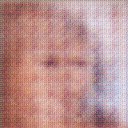
\includegraphics[width=150px]{500_fake_images/samples_5_405.png}%
\caption{A Close Up Of A Cat In A Bath Tub}%
\end{figure}

%
\end{document}